\chapter{Conclusion}

\label{chpt:Chapter5}

\chapterauthor{Nikolai G. Vetr}

\clearpage


\section{Does it work?}

Having finally arrived at the end of these chapters, we ask: does model-based inference of phylogeny from morphological data \textit{work}, and if not, what hope remains of its success? We have endeavored here to inject a greater dose of biological realism into the character evolutionary models used for phylogenetic inference, and so it is natural to ask whether that additional realism adequately captured vital aspects of the data-generating process not present in simpler models, and if those improvements were sufficient to retrieve phylogeny accurately and precisely. The trivial answer is that, to the extent that a statistical phylogenetic model may make predictions about its output that vary on the basis of tree topology or other parameters, those output can be used to make inference about those parameters in both Maximum Likelihood / Optimization and Bayesian frameworks. Assuming the model used for inference is not too poorly specified, probabilistic inferences should be well calibrated (Chapters \ref{chpt:Chapter2}, \ref{chpt:Chapter4}), with estimated nodal posterior probabilities trustworthy, which is to say accurate reflections of our uncertainty with respect to phylogenetic model parameters.

Probabilities rarely feel intuitive, however \citep{griffithsReconcilingIntuitionProbability2001}. We see high (e.g. $>$ 0.95) and low (e.g. $<$ 0.05) values as all but guaranteed, and are disproportionately surprised when their corresponding hypotheses come into conflict with independent inferential results or simulated ground-truth. Our surprise is even greater in point-estimated contexts --- when an algorithm whispers to us some hypothesis optimally satisfying the criteria we provide it, we balk at the thought of error, of inconsistency with our target reference \citep{collardHowReliableAre2000, gibbsSofttissueCharactersHigher2000}. But no statistical procedure guarantees perfection, and estimation error is entirely expected outside the limit of infinite data. It is through simulation that we may learn to temper our own expectations about what sorts of conclusions we are able to reach, training ourselves to be more skeptical of inferential results that we may more easily forgive them when their falsity is revealed. 

The methods developed here for inferring phylogeny from continuous and discrete morphological data appear to work when our expectations are so tempered. Plenty of information resides in continuous characters (\hyperref[chpt:Chapter2]{Chapter 2}), and it appears they can retrieve trees consistent with those obtained from molecular data commensurate with that information (\hyperref[chpt:Chapter3]{Chapter 3}). These trees are almost certainly all \textit{wrong}, which is to say that due to how diffusely the joint posterior distribution is spread, the reference or true tree is almost guaranteed never to have been sampled. But that is not to say that the inference procedure has failed us; perhaps more accurately, it is we who have failed the inference procedure, by failing to provide it with enough information that it not disappoint.

That said, it may be that fundamental limits will forever impede arbitrarily precise phylogenetic inference from morphological data. As described in the \hyperref[chpt:Chapter1]{Introduction}, morphological evolution is messy, and adequate models may quickly outpace in parameters both our computational resources and the extent of information we are able to squeeze from available datasets. Molecular sequences are a trove of (nearly) independently evolving loci, each possessing some small, insignificant signal of phylogeny, the pooling of which enables tremendously powerful inference under sophisticated phylogenetic models \citep{kapliPhylogeneticTreeBuilding2020}. In contrast to these thousands or millions of characters, morphological datasets rarely breach a hundred, and non-independence between characters in the presence of noise --- environmental, developmental, inferential, and measuremental --- quickly reduces the contribution of each marginal addition (Chapter \ref{chpt:Chapter2}), especially if novel parameters must be introduced to represent more complex morphological evolutionary processes. 

One may more easily imagine the impact of noise by imagining the rate matrix diagonalization procedure in Appendix \ref{app:App1} to not use Cholesky decomposition, but rather eigendecomposition. Absent noise, later eigenvectors (with smaller eigenvalues) correspond to equally informative axes of variation as earlier ones (Figure \ref{fig:noisyEigenvalues}a-b, $\sigma^2 = 0$). If covariance patterns in the noise are equivalent to that of the multivariate Brownian rate matrix, we likewise have not damaged ourselves much, merely extending terminal branch lengths by some small, if non-trivial amount (Figure \ref{fig:noisyEigenvalues}b). But if the noise is emitted from a distribution unlike the rate matrix, it may entirely obliterate the signal from those later eigenvectors if their eigenvalues are sufficiently small (Chapter \ref{chpt:Chapter2}, Figure \ref{fig:noisyEigenvalues}a). The story may even be more tragic than that portrayed (Figure \ref{fig:noisyEigenvalues}a), as the rate and noise matrices in these simulations are drawn from quite similar distributions, with the LKJ($\eta = 1$) concentrating most of its probability at high dimension near 0, implying the marginal distribution of each correlation coefficient to be beta(50, 50) stretched to the (-1,1) range. But morphological data at high dimension are likely not distributed according to flat correlation structure, and would feature far steeper scree plots than those implied by the flat LKJ (Figure \ref{fig:noisyEigenvalues}c), potentially disassociating projected trait values on later eigenvectors even more steeply and so more steeply diminishing the contribution of each subsequent measured trait. New techniques to characterize the human and primate morphomes will bring with them increasingly larger alignments of character data, but whether we will be able to use those data to our own satisfaction remains to be seen.

\begin{figure*}[h]
\centering
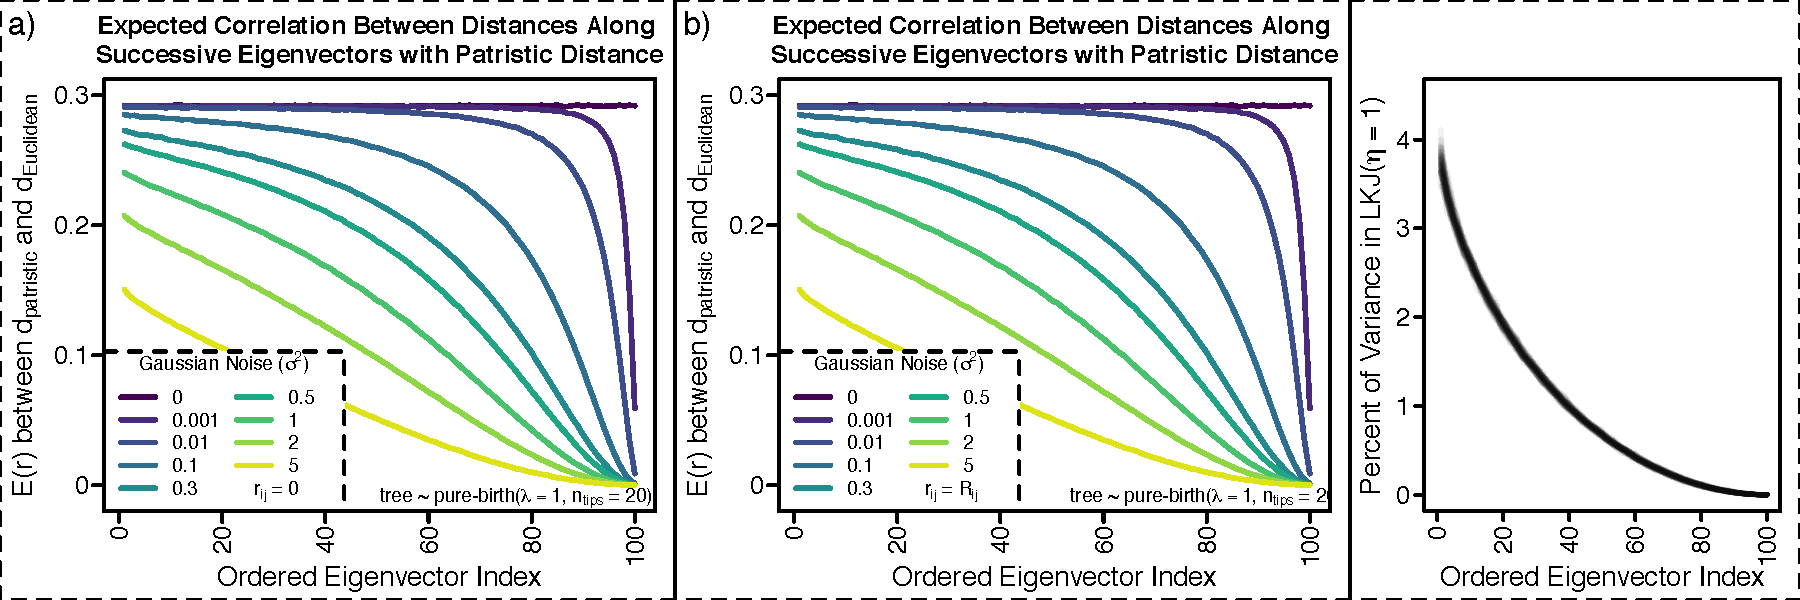
\includegraphics[width=160mm]{figures/noisydecay_of_association.pdf}
\caption[Association Between Euclidean Distances Along Eigenvectors and Patristic Distances]{Visualizing the association, here given as Pearson's r, between Euclidean distances between tips along succesive eigenvectors of a multivariate Brownian rate matrix and patristic distances on the tree on which those data evolved. For these figures, trees were first sampled from a pure birth distribution with 20 tips and $\lambda = 1$ (tree height $\approx 2.6 \pm 0.8, \mu \pm \sigma$). Then continuous character evolution was simulated on the sampled tree according to multivariate Brownian motion with a 100 x 100 rate matrix drawn from an LKJ($\eta = 1$). Tip characters were then perturbed with normally distributed noise and projected onto the eigenvectors of the Brownian rate matrix, and correlations between the distances separating each of the tips on each of these new axes and their corresponding patristic distances evaluated. In a), we see the expected correlation when the noise distribution is iid standard normal, as distinct from each sampled rate matrix. In b), noise is drawn from a multivariate normal with correlation structure equal to that of the multivariate Brownian rate matrix, effectively extending each tip by some amount $\sigma^2$. In c), the proportion of total variance corresponding to each eigenvector is shown, resulting in a distribution of scree plots implied by the LKJ.
\label{fig:noisyEigenvalues}
\label{overflow}}
\end{figure*}

\clearpage

\section{Limitunities}

Of course, we have far from exhausted our abilities to specify and fit models of morphological character evolution, and many opportunities await those willing to work past present limits. Joint inference represents the lowest hanging of these fruits, not only with respect to the use of full likelihoods, absent conditioning on erroneous optima (Chapter \ref{chpt:Chapter4}) estimated with imprecise approximations to our desired functions, but also through the pooling of information across molecular and morphological partitions. Much as fossils can tell us about morphological evolutionary processes across extant data \citep{slaterIntegratingFossilsMolecular2012}, so too can extant morphologies distributed across well-resolved molecular phylogenies tell us about the phylogenies of fossils. For those parts of the tree where nucleotide sequence (or other molecular) data are available, let \textit{them} sing their signals loud and clear, hopefully harmonizing across their thousands or millions of voices. Firm inference where available could then help to scaffold our understanding of local morphological evolutionary processes, as well as their variation. In those parts of the tree where molecular data are absent or unobtainable, hierarchical model structure will provide adaptively informative prior distributions for morphological evolutionary model parameters, that information present in those morphologies not need to spread itself too thin learning the location and shape of nuisance.

Model averaging may also help us to use more sophisticated models in proportion to the justification for their use. Developing more efficient jump moves \citep{huelsenbeckBayesianPhylogeneticModel2004} to move between high and low dimensional parameter spaces will allow us to sample from highly parameterized models according to their posterior probability, which will be lower according to the extent to which that model's marginal likelihood succeeds or fails to concentrate probability in favorable regions of the prior. With model averaging, phylogenetic inference can more organically explore the space of plausible models specified \textit{a priori}, averaging inference of focal model parameters pooled across those models (such as tree topology) to obtain a joint posterior distribution that makes use of multiple attempts to represent the underlying data-generating process. To the extent that simpler processes are preferred, the ensemble may visit them more, leveraging their simplicity to make more confident inference where possible.

On the model-specification front, the largest pitfalls of the preceding research are likely to pertain to assumptions of process homogeneity --- the constancy of some set of model parameters, such as trait-specific rates or between-trait correlations --- throughout the whole of our phylogenetic tree. Hierarchical model structure is the obvious solution. By specifying that some set of branch-specific model parameters are drawn from a common population of such parameters with some distribution, we can pool inference across branches while still accommodating branch-specific process heterogeneity. This strategy was employed in both chapters \ref{chpt:Chapter3} and \ref{chpt:Chapter4}, as well as during several side-projects undertaken during this dissertation, both mentioned (e.g. in Figure \ref{fig:OUPonds}) and unmentioned. Clever solutions exist for computing phylogenetic likelihoods in the face of such heterogeneity \citep[e.g.][]{caetanoEstimatingCorrelatedRates2019}, but where such solutions are not fast forthcoming, data augmentation may also be used over internal node states to dismantle a complex problem into a series of simpler ones (though not without its own difficulties, e.g. with respect to making efficient proposals). In this work, we strove to use populations and species for whom non-reticulate tree structure might apply with minor apologies. But population dynamics at sub-specific scales are likely to feature ample admixture, especially in such versatile, mobile, and promiscuous species as are found in our own lineage \citep{pruferCompleteGenomeSequence2014, durvasulaRecoveringSignalsGhost2020}. Accommodating reticulate network structure in the graphs we use to describe the evolution of morphological character data under multivariate Brownian motion \citep{pickrellInferencePopulationSplits2012, bastidePhylogeneticComparativeMethods2018} could be both intrinsically interesting and essential to accurate recovery of the underlying tree. And bounded Brownian motion processes, which are briefly mentioned in Appendix \ref{app:App3}, could also help to improve inference insofar as our taxa of interest might clash against hard limits in morphospace across the time scales separating them \citep{estesResolvingParadoxStasis2007}.

Finally, there exist a paucity of posterior predictive summary statistics \citep{gelmanPosteriorPredictiveAssessment1996} for use in model adequacy checks of morphological character evolutionary models, especially multivariate Brownian models. Elaboration of a plausible set of such statistics, as well as an exploration of their properties, could help to both identify when and where evolutionary models fail, as well as provide suggestions for how a model might be modified in order to better capture properties of our applied empirical context. 

Cliché though it may read, there remains much work to be done in the world of Bayesian morphological phylogenetics. In \textit{this} work, we explored the performance of multivariate Brownian models in a variety of simulated contexts, as well as with application to three empirical datasets drawn from the faces and dentitions of various monkeys and apes. Along the way, we developed both novel computational algorithms (such as those described in the appendices), as well as useful data visualization tools to characterize the informativeness of diffuse joint posterior distributions. The empirical results presented here are not intended to serve as final words on any outstanding questions, as might be expected given their focus on data able to be matched to molecular sequences. But they should serve to contextualize data analyses bereft of such convenience for paleontological samples whose use in the face of future discovery is all but guaranteed.

\clearpage


